\chapter{The VC Dimension}
\lecture{7}{30 Sep.}{}

\begin{prev}
    \autoref{thm:bounding} showed that a break point \(k\) caps the growth
    function by a polynomial, \(m_{\mathcal{H}}(N) \le B(N, k) =
    \sum_{i<k} \binom{N}{i}\), and \autoref{thm:vc} put \(m_{\mathcal{H}}(2N)\)
    where \(M\) used to be. Together: \(\Eout \approx \Ein\) is possible if
    \(m_{\mathcal{H}}(N)\) breaks somewhere and \(N\) is large enough.
\end{prev}

That conclusion depends on \(\mathcal{H}\) only through one number, its minimum
break point. This chapter gives that number a name (shifted by one), computes it
for perceptrons in any dimension, explains what it measures physically, and
then turns the VC bound around to read off what it says about model complexity
and about how much data is needed.

\section{Definition of VC Dimension}\label{sec:vc-def}

\source{slides p.2--7}

\subsection{Recap: More on Growth Function}

The last chapter ended with
\[
    m_{\mathcal{H}}(N) \text{ of break point } k
    \;\le\; B(N, k) = \underbrace{\sum_{i=0}^{k-1} \binom{N}{i}}_{\text{highest
    term } N^{k-1}} .
\]
The sum is awkward to carry around. Its highest term suggests replacing it by
the single power \(N^{k-1}\), and the two tables side by side show when that is
safe:

\begin{center}
    \solidrules
    \begin{tabular}{@{}cc|ccccc@{}}
        \toprule
        & & \multicolumn{5}{c}{\(k\)}\\
        & \(B(N, k)\) & \(1\) & \(2\) & \(3\) & \(4\) & \(5\)\\
        \midrule
        & \(1\) & \(1\) & \(2\) & \(2\) & \(2\) & \(2\)\\
        & \(2\) & \(1\) & \(3\) & \cellcolor{vcregion}\(4\)
        & \cellcolor{vcregion}\(4\) & \cellcolor{vcregion}\(4\)\\
        & \(3\) & \(1\) & \(4\) & \cellcolor{vcregion}\(7\)
        & \cellcolor{vcregion}\(8\) & \cellcolor{vcregion}\(8\)\\
        \(N\) & \(4\) & \(1\) & \(5\) & \cellcolor{vcregion}\(11\)
        & \cellcolor{vcregion}\(15\) & \cellcolor{vcregion}\(16\)\\
        & \(5\) & \(1\) & \(6\) & \cellcolor{vcregion}\(16\)
        & \cellcolor{vcregion}\(26\) & \cellcolor{vcregion}\(31\)\\
        & \(6\) & \(1\) & \(7\) & \cellcolor{vcregion}\(22\)
        & \cellcolor{vcregion}\(42\) & \cellcolor{vcregion}\(57\)\\
        \bottomrule
    \end{tabular}
    \qquad
    \begin{tabular}{@{}cc|ccccc@{}}
        \toprule
        & & \multicolumn{5}{c}{\(k\)}\\
        & \(N^{k-1}\) & \(1\) & \(2\) & \(3\) & \(4\) & \(5\)\\
        \midrule
        & \(1\) & \(1\) & \(1\) & \(1\) & \(1\) & \(1\)\\
        & \(2\) & \(1\) & \(2\) & \cellcolor{vcregion}\(4\)
        & \cellcolor{vcregion}\(8\) & \cellcolor{vcregion}\(16\)\\
        & \(3\) & \(1\) & \(3\) & \cellcolor{vcregion}\(9\)
        & \cellcolor{vcregion}\(27\) & \cellcolor{vcregion}\(81\)\\
        \(N\) & \(4\) & \(1\) & \(4\) & \cellcolor{vcregion}\(16\)
        & \cellcolor{vcregion}\(64\) & \cellcolor{vcregion}\(256\)\\
        & \(5\) & \(1\) & \(5\) & \cellcolor{vcregion}\(25\)
        & \cellcolor{vcregion}\(125\) & \cellcolor{vcregion}\(625\)\\
        & \(6\) & \(1\) & \(6\) & \cellcolor{vcregion}\(36\)
        & \cellcolor{vcregion}\(216\) & \cellcolor{vcregion}\(1296\)\\
        \bottomrule
    \end{tabular}
\end{center}

Cell by cell, the shaded entries on the right are at least those on the left.
Outside the shaded region the comparison fails: column \(k = 2\) has \(N + 1 >
N\), and row \(N = 1\) has \(2 > 1\). Hence

\begin{moral}
    Provably and loosely, for \(N \ge 2\), \(k \ge 3\),
    \[
        m_{\mathcal{H}}(N) \le B(N, k) = \sum_{i=0}^{k-1} \binom{N}{i}
        \le N^{k-1} .
    \]
\end{moral}

\begin{remark}
    The table is evidence, not a proof. One proof: for \(N \ge 2\), \(k \ge 3\),
    induct on \(k\). At \(k = 3\), \(1 + N + \frac{N(N-1)}{2} \le N^2\) is
    \((N-2)(N+1) \ge 0\) after doubling and rearranging, which holds for all
    \(N \ge 2\). Going from \(k\) to \(k+1\) adds \(\binom{N}{k} \le
    \frac{N^{k}}{k!} \le N^{k} - N^{k-1}\) whenever \(N \ge 2\) and \(k \ge 2\),
    since then \(N^{k-1}(N - 1) \ge N^{k}/2 \ge N^{k}/k!\).
\end{remark}

\subsection{Recap: More on Vapnik--Chervonenkis (VC) Bound}

Chaining the VC bound with this estimate, for any \(g = \mathcal{A}(\mathcal{D})
\in \mathcal{H}\) and a `statistical' large \(\mathcal{D}\), for \(N \ge 2\),
\(k \ge 3\):
\begin{align*}
    \mathbb{P}_{\mathcal{D}}\left[ \abs{\Ein(g) - \Eout(g)} > \epsilon \right]
    &\le \mathbb{P}_{\mathcal{D}}\left[ \exists h \in \mathcal{H} \text{ s.t. }
    \abs{\Ein(h) - \Eout(h)} > \epsilon \right]\\
    &\le 4 m_{\mathcal{H}}(2N) \exp \left( -\frac{1}{8} \epsilon^2 N \right)\\
    &\overset{\text{if } k \text{ exists}}{\le}
    4 (2N)^{k-1} \exp \left( -\frac{1}{8} \epsilon^2 N \right) .
\end{align*}
The first step holds because \(g\) is one of the \(h\); the last applies the
moral above at \(2N\) points. The subscript \(\mathcal{D}\) is a reminder that
the probability is over the draw of the data. Reading the chain as a recipe for
learning:

\begin{center}
    \begin{tabular}{@{}rlr@{}}
        if & (1)~\(m_{\mathcal{H}}(N)\) breaks at \(k\)
        & (good \(\mathcal{H}\))\\
        & (2)~\(N\) large enough & (good \(\mathcal{D}\))\\
        \multicolumn{2}{@{}l}{\(\implies\) probably generalized
        `\(\Eout \approx \Ein\)', and} & \\
        if & (3)~\(\mathcal{A}\) picks a \(g\) with small \(\Ein\)
        & (good \(\mathcal{A}\))\\
        \multicolumn{2}{@{}l}{\(\implies\) probably learned!}
        & (:-) good luck)
    \end{tabular}
\end{center}

The first two conditions are what the theory has been building; the third is an
optimisation problem, and is the subject of \emph{How can machines learn?}

\subsection{VC Dimension}

The chain carries the exponent \(k - 1\) everywhere, so it is natural to name
that number directly: the formal name of the \emph{maximum non}-break point.

\begin{definition}[VC dimension]\label{def:vc}
    The \vocab{VC dimension} of \(\mathcal{H}\), denoted \(\dvc(\mathcal{H})\), is
    the
    \[
        \text{largest } N \text{ for which } m_{\mathcal{H}}(N) = 2^N .
    \]
    \begin{itemize}
        \item It is the \emph{most} inputs \(\mathcal{H}\) can shatter.
        \item \(\dvc = \text{`minimum } k\text{'} - 1\).
    \end{itemize}
\end{definition}

If \(m_{\mathcal{H}}(N) = 2^N\) for every \(N\) there is no break point and
\(\dvc = \infty\). The definition asks for \emph{some} set of \(N\) inputs to be
shattered, never all of them. Unwinding it,
\begin{align*}
    N \le \dvc &\implies \mathcal{H} \text{ can shatter some } N \text{ inputs},\\
    k > \dvc &\implies k \text{ is a break point for } \mathcal{H} .
\end{align*}
The second line is the one the bounds use: with \(k = \dvc + 1\), the moral of
the recap becomes

\begin{moral}
    If \(N \ge 2\), \(\dvc \ge 2\), then \(m_{\mathcal{H}}(N) \le N^{\dvc}\).
\end{moral}

\subsection{The Four VC Dimensions}

Reading off the four hypothesis sets of \autoref{sec:effective-hyp}, with a
largest shattered configuration drawn next to each:

\begin{center}
    \solidrules
    \begin{adjustbox}{max width=\textwidth}
        \begin{tabular}{@{}l|c|c|l@{}}
            \toprule
            \(\mathcal{H}\) & \(\dvc\) & largest shattered inputs
            & \(m_{\mathcal{H}}(N)\)\\
            \midrule
            positive rays & \(1\)
            & \tikz[baseline=-0.6ex]{\fill (0,0) circle (1.4pt);}
            & \(N + 1\)\\
            positive intervals & \(2\)
            & \tikz[baseline=-0.6ex]{\fill (0,0) circle (1.4pt);
                \fill (0.3,0) circle (1.4pt);}
            & \(\tfrac{1}{2} N^2 + \tfrac{1}{2} N + 1\)\\
            convex sets & \(\infty\)
            & \tikz[baseline=(current bounding box.center)]{%
                \foreach \t in {0,40,...,320}
                    {\fill (\t+20:0.42) circle (1.1pt);}
                \node[font=\tiny, above] at (0,0.45) {up};
                \node[font=\tiny, below] at (0,-0.45) {bottom};}
            & \(2^N\)\\
            2D perceptrons & \(3\)
            & \tikz[baseline=(current bounding box.center)]{%
                \fill (0.15,0.26) circle (1.4pt);
                \fill (0,0) circle (1.4pt);
                \fill (0.3,0) circle (1.4pt);}
            & \(\le N^3\) for \(N \ge 2\)\\
            \bottomrule
        \end{tabular}
    \end{adjustbox}
\end{center}

Each \(\dvc\) is the minimum break point of the previous chapters minus one:
\(2 - 1\), \(3 - 1\), none, \(4 - 1\). The convex-set picture is the circle
configuration of \autoref{prop:convex}, which is shattered for every \(N\). For
2D perceptrons we still do not know \(m_{\mathcal{H}}(N)\) exactly, but
\(\dvc = 3\) is enough to get \(m_{\mathcal{H}}(N) \le N^3\).

\begin{moral}
    Good: finite \(\dvc\).
\end{moral}

\subsection{VC Dimension and Learning}

\begin{moral}
    Finite \(\dvc\) \(\implies\) \(g\) `will' generalize (\(\Eout(g) \approx
    \Ein(g)\)).
\end{moral}

What is remarkable is what the guarantee does \emph{not} need:

\begin{itemize}
    \item regardless of learning algorithm \(\mathcal{A}\);
    \item regardless of input distribution \(P\);
    \item regardless of target function \(f\).
\end{itemize}

In the learning flow, those three boxes can be greyed out; the guarantee
depends only on the hypothesis set and the size of the training set.

\begin{center}
    \begin{adjustbox}{max width=\textwidth}
        \begin{tikzpicture}
            \node[mlbox, minimum width=4.4cm, draw=black!25, text=black!40]
                (f) at (0,2.5)
                {unknown target function\\
                 \(f\colon \mathcal{X} \to \mathcal{Y}\)\\[2pt]
                 {\scriptsize (ideal credit approval formula)}};
            \node[mlbox, minimum width=2.6cm, draw=black!25, text=black!40]
                (P) at (5.4,2.5) {unknown\\\(P\) on \(\mathcal{X}\)};
            \node[mlbox, minimum width=5.2cm] (D) at (0,0)
                {training examples\\
                 \(\mathcal{D}\colon (\bm{x}_1, y_1), \dots , (\bm{x}_N, y_N)\)\\[2pt]
                 {\scriptsize (historical records in bank)}};
            \node[mlop, minimum width=2.4cm, fill=black!3, draw=black!25,
                text=black!40] (A) at (5.4,0)
                {learning\\algorithm\\\(\mathcal{A}\)};
            \node[mlbox, minimum width=4.4cm] (g) at (10.2,0)
                {final hypothesis\\\(g \approx f\)\\[2pt]
                 {\scriptsize (`learned' formula to be used)}};
            \node[mlbox, minimum width=3.4cm, draw=red!70!black, very thick]
                (H) at (5.4,-2.4)
                {hypothesis set\\\(\mathcal{H}\)\\[2pt]
                 {\scriptsize (set of candidate formulas)}};
            \node[align=center, font=\small] at (10.2,-2.4)
                {\textcolor{orange!85!black}{\textbf{`worst case'}} guarantee\\
                 on generalization};
            \draw[mlarrow, draw=black!30] (f) -- (D);
            \draw[mlarrow, draw=black!30, dashed] (P) -- (D)
                node[pos=0.58, font=\scriptsize, fill=white, inner sep=1.5pt,
                text=black!40] {\(\bm{x}_1, \bm{x}_2, \dots , \bm{x}_N\)};
            \draw[mlarrow, draw=black!30, dashed] (P.east) -| (g.north)
                node[pos=0.25, above, font=\scriptsize, text=black!40]
                {\(\bm{x}\)};
            \draw[mlarrow] (D) -- (A);
            \draw[mlarrow] (A) -- (g);
            \draw[mlarrow] (H) -- (A);
        \end{tikzpicture}
    \end{adjustbox}
\end{center}

`Worst case' is the price of that generality: the bound has to hold for the
least favourable \(\mathcal{A}\), \(P\) and \(f\) at once, which is one reason
it will turn out loose (\autoref{sec:vc-interpret}).

\begin{exercise}[Fun Time]
    If there is a set of \(N\) inputs that cannot be shattered by
    \(\mathcal{H}\). Based only on this information, what can we conclude
    about \(\dvc(\mathcal{H})\)?
    \begin{enumerate*}[(1)]
        \item \(\dvc(\mathcal{H}) > N\); \item \(\dvc(\mathcal{H}) = N\);
        \item \(\dvc(\mathcal{H}) < N\); \item no conclusion can be made.
    \end{enumerate*}
\end{exercise}

\begin{proof}[Reference Answer]
    (4). It is possible that there is another set of \(N\) inputs that can be
    shattered, which means \(\dvc \ge N\). It is also possible that no set of
    \(N\) inputs can be shattered, which means \(\dvc < N\). Neither case can
    be ruled out by one non-shattering set. (Three collinear points, which
    no line shatters, are the example: they say nothing against
    \(\dvc = 3\) for 2D perceptrons.)
\end{proof}

\section{VC Dimension of Perceptrons}\label{sec:vc-perceptron}

\source{slides p.8--16}

\subsection{2D PLA Revisited}

With \(\dvc\) in hand, the story of 2D PLA can finally be closed. Two
independent chains lead to the same place:

\begin{center}
    \begin{adjustbox}{max width=\textwidth}
        \begin{tikzpicture}[font=\small, node distance=0pt]
            \node[text=red!80!black] (sep) at (0,3.2) {linearly separable
                \(\mathcal{D}\)};
            \node[text=red!80!black] (conv) at (0,2.2) {PLA can converge};
            \node[text=red!80!black] (ein) at (0,0) {\(\Ein(g) = 0\)};
            \node[text=blue!80!black] (iid) at (6,3.2) {with \(\bm{x}_n \sim P\)
                and \(y_n = f(\bm{x}_n)\)};
            \node[text=blue!80!black, fill=blue!10, inner sep=2pt] (vc)
                at (6,2.2) {\(\mathbb{P}\left[ \abs{\Ein(g) - \Eout(g)} >
                \epsilon \right] \le \dots\) by \(\dvc = 3\)};
            \node[text=blue!80!black] (gen) at (6,0)
                {\(\Eout(g) \approx \Ein(g)\)};
            \node[text=orange!85!black] (out) at (3,-1)
                {\(\Eout(g) \approx 0\) :-)};
            \draw[mlarrow, draw=red!80!black] (sep) -- (conv);
            \draw[mlarrow, draw=red!80!black] (conv) -- (ein)
                node[midway, left] {\(T\) large};
            \draw[mlarrow, draw=blue!80!black] (iid) -- (vc);
            \draw[mlarrow, draw=blue!80!black] (vc) -- (gen)
                node[midway, right] {\(N\) large};
            \draw[mlarrow, draw=orange!85!black] (ein) -- (out);
            \draw[mlarrow, draw=orange!85!black] (gen) -- (out);
        \end{tikzpicture}
    \end{adjustbox}
\end{center}

The left chain is optimisation (\autoref{sec:pla-guarantee}): after enough
iterations \(T\), PLA makes no mistake on \(\mathcal{D}\). The right chain is
generalisation: with enough examples \(N\), \(\Ein\) is close to \(\Eout\) for
any line, including the one PLA returns. Together they give \(\Eout(g) \approx
0\).

\begin{question}
    General PLA for \(\bm{x}\) with more than \(2\) features?
\end{question}

\subsection{VC Dimension of Perceptrons}

What is known so far:

\begin{itemize}
    \item 1D perceptron (pos/neg rays): \(\dvc = 2\);
    \item 2D perceptrons: \(\dvc = 3\)
    \begin{itemize}
        \item \(\dvc \ge 3\): \tikz[baseline=0.3ex, x=0.3cm, y=0.3cm]{%
            \fill (0.5,0.9) circle (1.4pt); \fill (0,0) circle (1.4pt);
            \fill (1,0) circle (1.4pt);} can be shattered;
        \item \(\dvc \le 3\): \tikz[baseline=0.6ex, x=0.3cm, y=0.3cm]{%
            \dmarkat{1}{2}{o}\dmarkat{0}{1}{x}\dmarkat{2}{1}{x}%
            \dmarkat{1}{0}{o}} no four inputs can be shattered;
    \end{itemize}
    \item \(d\)-D perceptrons: \(\dvc \overset{?}{=} d + 1\).
\end{itemize}

The first two fit the guess \(d + 1\): \(1 + 1\) and \(2 + 1\). The extra
\(1\) is the threshold, which \autoref{sec:perceptron-set} absorbed as
\(w_0\) with the constant coordinate \(x_0 = 1\), so a \(d\)-D perceptron really
has \(d + 1\) weights. Proving \(\dvc = d + 1\) takes two steps:

\begin{itemize}
    \item \(\dvc \ge d + 1\);
    \item \(\dvc \le d + 1\).
\end{itemize}

The two steps need different kinds of evidence, as the next two quizzes make
precise.

\begin{exercise}[Extra Fun Time]
    What statement below shows that \(\dvc \ge d + 1\)?
    \begin{enumerate}[(1)]
        \item There are some \(d + 1\) inputs we can shatter.
        \item We can shatter any set of \(d + 1\) inputs.
        \item There are some \(d + 2\) inputs we cannot shatter.
        \item We cannot shatter any set of \(d + 2\) inputs.
    \end{enumerate}
\end{exercise}

\begin{proof}[Reference Answer]
    (1). \(\dvc\) is the maximum \(N\) such that \(m_{\mathcal{H}}(N) = 2^N\),
    and \(m_{\mathcal{H}}(N)\) is the most number of dichotomies of \(N\)
    inputs. So if we can find \(2^{d+1}\) dichotomies on \emph{some} \(d + 1\)
    inputs, \(m_{\mathcal{H}}(d + 1) = 2^{d+1}\) and hence \(\dvc \ge d + 1\).
    (2) is also sufficient but asks for far more than needed --- and is false
    for perceptrons, as collinear points show.
\end{proof}

\subsection{\texorpdfstring{\(\dvc \ge d + 1\)}{dVC >= d + 1}}

By the quiz, it is enough that there are \emph{some} \(d + 1\) inputs we can
shatter. Pick some `trivial' inputs: the origin and the \(d\) unit vectors,
each with the constant coordinate \(x_0 = 1\) in front. As the rows of a
matrix,
\[
    \mathrm{X} =
    \begin{bmatrix}
        \text{---}\; \bm{x}_1^\top \;\text{---}\\
        \text{---}\; \bm{x}_2^\top \;\text{---}\\
        \text{---}\; \bm{x}_3^\top \;\text{---}\\
        \vdots\\
        \text{---}\; \bm{x}_{d+1}^\top \;\text{---}
    \end{bmatrix}
    =
    \begin{bmatrix}
        1 & 0 & 0 & \dots & 0\\
        1 & 1 & 0 & \dots & 0\\
        1 & 0 & 1 & & 0\\
        \vdots & \vdots & & \ddots & 0\\
        1 & 0 & \dots & 0 & 1
    \end{bmatrix} .
\]
Visually in 2D these are the three points \tikz[baseline=0.3ex, x=0.3cm,
y=0.3cm]{\fill[orange] (0,1) circle (1.4pt); \fill[orange] (0,0) circle
(1.4pt); \fill[orange] (1,0) circle (1.4pt);} at \((0,0)\), \((1,0)\) and
\((0,1)\). Note: \(\mathrm{X}\) is \(\bm{(d+1) \times (d+1)}\) and
\textbf{invertible} --- subtracting the first row from every other row leaves
the identity matrix.

\begin{remark}
    The \(d + 1\) inputs are points of \(\mathbb{R}^d\): the origin
    \(\bm{0}\) and the \(d\) standard unit vectors \(\bm{e}_1, \dots ,
    \bm{e}_d\), where \(\bm{e}_i\) has \(1\) in its \(i\)-th entry and \(0\)
    elsewhere. So \(\bm{x}_1 = (1, \bm{0})\) and \(\bm{x}_{i+1} = (1,
    \bm{e}_i)\) for \(i = 1, \dots , d\). The first column of \(\mathrm{X}\)
    is not part of the data: it is the bias coordinate \(x_0 = 1\)
    (\autoref{sec:perceptron-set}). This is why a \(d\)-D
    perceptron works with \((d+1)\)-dimensional vectors, and why
    \(\mathrm{X}\) is square.
\end{remark}

\subsection{Can We Shatter \texorpdfstring{\(\mathrm{X}\)}{X}?}

To shatter \(\mathrm{X}\) means: for any
\(\bm{y} = (y_1, \dots , y_{d+1})^\top\) with entries \(\pm 1\), find \(\bm{w}\)
such that \(\sign(\mathrm{X} \bm{w}) = \bm{y}\), the \(n\)-th entry of
\(\mathrm{X}\bm{w}\) being \(\bm{w}^\top \bm{x}_n\). Demanding the signs is
hard; demanding the values is easy, because \(\mathrm{X}\) is invertible:
\[
    \sign(\mathrm{X} \bm{w}) = \bm{y}
    \quad\Longleftarrow\quad
    \mathrm{X} \bm{w} = \bm{y}
    \quad\overset{\mathrm{X} \text{ invertible!}}{\iff}\quad
    \bm{w} = \mathrm{X}^{-1} \bm{y} .
\]
The first implication holds because \(\sign(\pm 1) = \pm 1\). So every one of
the \(2^{d+1}\) label vectors is realised by some perceptron:

\begin{moral}
    `Special' \(\mathrm{X}\) can be shattered \(\implies\) \(\dvc \ge d + 1\).
\end{moral}

\begin{exercise}[Extra Fun Time]
    What statement below shows that \(\dvc \le d + 1\)?
    \begin{enumerate}[(1)]
        \item There are some \(d + 1\) inputs we can shatter.
        \item We can shatter any set of \(d + 1\) inputs.
        \item There are some \(d + 2\) inputs we cannot shatter.
        \item We cannot shatter any set of \(d + 2\) inputs.
    \end{enumerate}
\end{exercise}

\begin{proof}[Reference Answer]
    (4). \(\dvc\) is the maximum \(N\) such that \(m_{\mathcal{H}}(N) = 2^N\),
    and \(m_{\mathcal{H}}(N)\) is the most number of dichotomies of \(N\)
    inputs. So if we cannot find \(2^{d+2}\) dichotomies on \emph{any}
    \(d + 2\) inputs (i.e.\ break point), \(m_{\mathcal{H}}(d + 2) < 2^{d+2}\)
    and hence \(\dvc < d + 2\). That is, \(\dvc \le d + 1\). Statement (3) is the
    trap of the Fun Time in \autoref{sec:vc-def}: one bad set proves nothing.
\end{proof}

The upper bound is therefore the harder half: a single well-chosen example no
longer suffices, and the argument must work for \emph{every} set of \(d + 2\)
inputs.

\subsection{\texorpdfstring{\(\dvc \le d + 1\)}{dVC <= d + 1}: A 2D Special
Case}

Start with four inputs in 2D, the corners of the unit square:
\[
    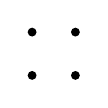
\begin{tikzpicture}[baseline=(current bounding box.center), x=0.55cm,
        y=0.55cm]
        \foreach \p in {(0,0),(1,0),(0,1),(1,1)}{\fill \p circle (1.6pt);}
    \end{tikzpicture}
    \qquad
    \mathrm{X} =
    \begin{bmatrix}
        \text{---}\; \bm{x}_1^\top \;\text{---}\\
        \text{---}\; \bm{x}_2^\top \;\text{---}\\
        \text{---}\; \bm{x}_3^\top \;\text{---}\\
        \text{---}\; \bm{x}_4^\top \;\text{---}
    \end{bmatrix}
    =
    \begin{bmatrix}
        1 & 0 & 0\\
        1 & 1 & 0\\
        1 & 0 & 1\\
        1 & 1 & 1
    \end{bmatrix} .
\]
So \(\bm{x}_1\) is the lower-left corner, \(\bm{x}_2\) lower-right,
\(\bm{x}_3\) upper-left, \(\bm{x}_4\) upper-right. Four rows in a
three-dimensional space must be linearly dependent, and here the dependence is
visible: \(\bm{x}_4 = \bm{x}_2 + \bm{x}_3 - \bm{x}_1\). Now label
\(\bm{x}_2, \bm{x}_3\) as \(\circ\) and \(\bm{x}_1\) as \(\times\):
\[
    \begin{tikzpicture}[baseline=(current bounding box.center), x=0.55cm,
        y=0.55cm]
        \dmarkat{0}{1}{o}
        \node[font=\bfseries] at (1,1) {?};
        \dmarkat{0}{0}{x}
        \dmarkat{1}{0}{o}
    \end{tikzpicture}
    \qquad
    \text{\colorbox{Purple!15}{\textbf{?} cannot be \(\times\)}}
\]
because for every \(\bm{w}\) producing these three labels,
\[
    \bm{w}^\top \bm{x}_4
    = \underbrace{\bm{w}^\top \bm{x}_2}_{\circ}
    + \underbrace{\bm{w}^\top \bm{x}_3}_{\circ}
    - \underbrace{\bm{w}^\top \bm{x}_1}_{\times} > 0 :
\]
the first two terms are positive, and subtracting a negative one only adds.
This is the XOR dichotomy again, now explained algebraically.

\begin{moral}
    Linear dependence restricts dichotomy.
\end{moral}

\subsection{\texorpdfstring{\(\dvc \le d + 1\)}{dVC <= d + 1}: The
\texorpdfstring{\(d\)}{d}-D General Case}

By the Extra Fun Time above, proving \(\dvc \le d + 1\) means proving that
\(m_{\mathcal{H}}(d + 2) < 2^{d+2}\): \emph{no} set of \(d + 2\) inputs can be
shattered. One bad configuration, such as the square, is not enough; the
argument has to work for every choice of \(d + 2\) inputs. So take
\emph{any} \(d + 2\) inputs, as rows of
\[
    \mathrm{X} =
    \begin{bmatrix}
        \text{---}\; \bm{x}_1^\top \;\text{---}\\
        \text{---}\; \bm{x}_2^\top \;\text{---}\\
        \vdots\\
        \text{---}\; \bm{x}_{d+1}^\top \;\text{---}\\
        \text{---}\; \bm{x}_{d+2}^\top \;\text{---}
    \end{bmatrix} .
\]
There are more rows (\(d + 2\)) than columns (\(d + 1\)), so the rows are
linearly dependent: some row is a combination of the others. Relabelling so
that this row is the last one,
\[
    \bm{x}_{d+2} = \textcolor{blue!80!black}{a_1} \bm{x}_1
    + \textcolor{red!80!black}{a_2} \bm{x}_2 + \dots
    + \textcolor{red!80!black}{a_{d+1}} \bm{x}_{d+1} ,
    \qquad \text{some } a_i \text{ non-zero}.
\]

\begin{itemize}
    \item Can you generate \((\sign(a_1), \sign(a_2), \dots ,
        \sign(a_{d+1}), \times)\)? If so, what \(\bm{w}\)?
        \[
            \bm{w}^\top \bm{x}_{d+2}
            = \textcolor{blue!80!black}{a_1}
            \underbrace{\bm{w}^\top \bm{x}_1}_{\circ}
            + \textcolor{red!80!black}{a_2}
            \underbrace{\bm{w}^\top \bm{x}_2}_{\times}
            + \dots + \textcolor{red!80!black}{a_{d+1}}
            \underbrace{\bm{w}^\top \bm{x}_{d+1}}_{\times}
            > 0 \quad\text{(contradiction!)}
        \]
\end{itemize}

The braces show a typical sign pattern, \(a_1 > 0\) and the rest negative.
Note the direction of the argument. To show that the \(d + 2\) inputs are
\emph{not} shattered, it is not enough to find one \(\bm{w}\) with a bad
output; we must exhibit one dichotomy that \emph{no} \(\bm{w}\) produces. The
dichotomy is chosen from the coefficients \(a_i\), and then every \(\bm{w}\)
that gets the first \(d + 1\) labels right is shown to be forced to say
\(\circ\) on \(\bm{x}_{d+2}\).

\begin{lemma}[Linear dependence blocks a dichotomy]\label{lem:dep-block}
    Let \(\bm{x}_1, \dots , \bm{x}_{d+2} \in \mathbb{R}^{d+1}\) be any
    \(d + 2\) inputs (bias coordinate \(x_0 = 1\) included). Then some
    dichotomy \((y_1, \dots , y_{d+2})\) is not \((\sign(\bm{w}^\top
    \bm{x}_1), \dots , \sign(\bm{w}^\top \bm{x}_{d+2}))\) for any
    \(\bm{w} \in \mathbb{R}^{d+1}\).
\end{lemma}

\begin{proof}
    \emph{Step 1: the coefficients.} \(d + 2\) vectors in
    \(\mathbb{R}^{d+1}\) are linearly dependent, so \(\sum_{i=1}^{d+2} c_i
    \bm{x}_i = \bm{0}\) for some \(c_i\) not all zero. Pick \(j\) with \(c_j
    \ne 0\), divide by \(-c_j\), and renumber so that \(j = d + 2\):
    \[
        \bm{x}_{d+2} = \sum_{i=1}^{d+1} a_i \bm{x}_i .
    \]
    At least one \(a_i\) is non-zero, since otherwise \(\bm{x}_{d+2} =
    \bm{0}\), impossible because its first coordinate is \(x_0 = 1\).

    \emph{Step 2: the dichotomy.} Define
    \[
        y_i = \begin{cases}
            \sign(a_i) & \text{if } a_i \ne 0,\\
            +1 \text{ (say; any value works)} & \text{if } a_i = 0,
        \end{cases}
        \qquad i = 1, \dots , d + 1, \qquad y_{d+2} = -1 .
    \]

    \emph{Step 3: no \(\bm{w}\) produces it.} Suppose \(\bm{w}\) gives
    \(\sign(\bm{w}^\top \bm{x}_i) = y_i\) for \(i = 1, \dots , d + 1\). Take
    the inner product of Step 1 with \(\bm{w}\):
    \[
        \bm{w}^\top \bm{x}_{d+2} = \sum_{i=1}^{d+1} a_i \,
        (\bm{w}^\top \bm{x}_i) .
    \]
    Look at each term. If \(a_i = 0\) the term is \(0\). If \(a_i \ne 0\),
    then \(\bm{w}^\top \bm{x}_i\) has the sign \(y_i = \sign(a_i)\), in
    particular it is non-zero, so \(a_i (\bm{w}^\top \bm{x}_i)\) is a product
    of two non-zero numbers of the same sign, hence \(> 0\). Every term is
    \(\ge 0\) and at least one is \(> 0\), so \(\bm{w}^\top \bm{x}_{d+2} >
    0\) and \(\sign(\bm{w}^\top \bm{x}_{d+2}) = +1 \ne y_{d+2}\).

    So every \(\bm{w}\) that is right on the first \(d + 1\) inputs is wrong
    on the last, and \((y_1, \dots , y_{d+2})\) is never produced.
\end{proof}

The \(2\)D special case above is the instance \(d = 2\), \(\bm{x}_4 =
\bm{x}_2 + \bm{x}_3 - \bm{x}_1\): \(a = (-1, 1, 1)\), so the blocked dichotomy
is \((\times, \circ, \circ, \times)\). Since the lemma holds for \emph{any}
\(d + 2\) inputs, no set of \(d + 2\) inputs is shattered: \(m_{\mathcal{H}}(d
+ 2) < 2^{d+2}\), i.e.\ \(d + 2\) is a break point, which is statement (4) of
the last Extra Fun Time.

\begin{moral}
    `General' \(\mathrm{X}\) no-shatter \(\implies\) \(\dvc \le d + 1\).
\end{moral}

With both steps done:

\begin{theorem}[VC dimension of perceptrons]\label{thm:vc-perceptron}
    For \(d\)-D perceptrons, \(\dvc = d + 1\).
\end{theorem}

\begin{exercise}[Fun Time]
    Based on the proof above, what is \(\dvc\) of 1126-D perceptrons?
    \begin{enumerate*}[(1)]
        \item \(1024\); \item \(1126\); \item \(1127\); \item \(6211\).
    \end{enumerate*}
\end{exercise}

\begin{proof}[Reference Answer]
    (3). \(1126 + 1 = 1127\). Well, too much fun for this section! :-)
\end{proof}

\section{Physical Intuition of VC Dimension}\label{sec:vc-intuition}

\source{slides p.17--20}

\autoref{thm:vc-perceptron} says a perceptron has \(\dvc\) equal to its number of
weights. That is suggestive enough to ask what \(\dvc\) is measuring in general.

\subsection{Degrees of Freedom}

\begin{center}
    \begin{adjustbox}{max width=\textwidth}
        \begin{tikzpicture}
            \foreach \t [count=\i from 0] in {4,9,15,10,5}{
                \dialknob{2.1*\i}{2.1}{\t}}
            \foreach \t [count=\i from 0] in {16,17,14,2,3}{
                \dialknob{2.1*\i}{0}{\t}}
        \end{tikzpicture}
    \end{adjustbox}

    {\footnotesize (modified from the work of Hugues Vermeiren on
    \nolinkurl{http://www.texample.net})}
\end{center}

Think of a hypothesis as a machine with knobs, each weight being one knob. The
three quantities met so far are three ways of counting what the knobs can do:

\begin{itemize}
    \item hypothesis parameters \(\bm{w} = (w_0, w_1, \dots , w_d)\):
        \textbf{create degrees of freedom};
    \item hypothesis quantity \(M = \abs{\mathcal{H}}\): `analog' degrees of
        freedom;
    \item hypothesis `power' \(\dvc = d + 1\): \textbf{effective `binary'
        degrees of freedom}.
\end{itemize}

\(M\) counts every knob setting, and is infinite as soon as a knob turns
continuously. \(\dvc\) counts only how many inputs the knobs can label
independently in \emph{every} possible way --- how many free binary choices
the knobs really control.

\begin{moral}
    \(\dvc(\mathcal{H})\): powerfulness of \(\mathcal{H}\).
\end{moral}

\subsection{Two Old Friends}

The hypothesis sets of \autoref{sec:effective-hyp} fit the same picture.

\begin{center}
    \begin{tikzpicture}[font=\small]
        % positive rays
        \node[anchor=west, font=\small\bfseries] at (-0.4,1.35)
            {Positive Rays (\(\dvc = 1\))};
        \draw[black!70] (0,0) -- (8,0);
        \node[text=red!80!black] at (1.8,0.35) {\(h(x) = -1\)};
        \draw[blue!70!black, thick] (4,-0.12) -- (4,0.55);
        \draw[-{Stealth[length=2mm]}, blue!70!black, thick] (4,0.4) -- (7.6,0.4);
        \node[text=blue!70!black] at (5.8,0.7) {\(h(x) = +1\)};
        \node[below, text=blue!70!black] at (4,-0.1) {\(a\)};
        \node[text=Purple] at (4,-0.75) {free parameters: \(a\)};
        % positive intervals
        \begin{scope}[yshift=-2.6cm]
            \node[anchor=west, font=\small\bfseries] at (-0.4,1.35)
                {Positive Intervals (\(\dvc = 2\))};
            \draw[black!70] (0,0) -- (8,0);
            \node[text=red!80!black] at (1.5,0.35) {\(h(x) = -1\)};
            \draw[blue!70!black, thick] (3,-0.12) -- (3,0.55);
            \draw[blue!70!black, thick] (5.2,-0.12) -- (5.2,0.55);
            \draw[{Stealth[length=2mm]}-{Stealth[length=2mm]}, blue!70!black,
                thick] (3,0.4) -- (5.2,0.4);
            \node[text=blue!70!black] at (4.1,0.72) {\(h(x) = +1\)};
            \node[text=red!80!black] at (6.6,0.35) {\(h(x) = -1\)};
            \node[below, text=blue!70!black] at (3,-0.1) {\(\ell\)};
            \node[below, text=blue!70!black] at (5.2,-0.1) {\(r\)};
            \node[text=Purple] at (4,-0.75) {free parameters: \(\ell, r\)};
        \end{scope}
    \end{tikzpicture}
\end{center}

One threshold, one binary degree of freedom; two endpoints, two. This suggests

\begin{moral}
    Practical rule of thumb: \(\dvc \approx \#\)free parameters (but not
    always).
\end{moral}

`Not always' in both directions: parameters can be redundant (\(h(x) =
\sign(w_1 w_2 x)\) has two parameters but only the sign of the product
matters), and a single parameter can be enormously powerful (\(h(x) =
\sign(\sin(\alpha x))\) has one parameter and \(\dvc = \infty\)).

\subsection{\texorpdfstring{\(M\)}{M} and \texorpdfstring{\(\dvc\)}{dVC}}

Copied from \autoref{sec:recap-preview} :-), the two central questions are:

\begin{enumerate}[(1)]
    \item can we make sure that \(\Eout(g)\) is close enough to \(\Ein(g)\)?
    \item can we make \(\Ein(g)\) small enough?
\end{enumerate}

\(\dvc\) now plays exactly the role \(M\) played there, with \(M\) replaced by
the polynomial \((2N)^{\dvc}\):

\begin{center}
    \solidrules
    \begin{tabular}{@{}l|l|l@{}}
        \toprule
        & (1) \(\Eout \approx \Ein\)? & (2) \(\Ein\) small?\\
        \midrule
        small \(M\) & Yes!, \(\mathbb{P}[\textbf{BAD}] \le 2 \cdot M \cdot
        \exp(\dots)\) & No!, too few choices\\
        large \(M\) & No!, \(\mathbb{P}[\textbf{BAD}] \le 2 \cdot M \cdot
        \exp(\dots)\) & Yes!, many choices\\
        \midrule
        small \(\dvc\) & Yes!, \(\mathbb{P}[\textbf{BAD}] \le 4 \cdot
        (2N)^{\dvc} \cdot \exp(\dots)\) & No!, too limited power\\
        large \(\dvc\) & No!, \(\mathbb{P}[\textbf{BAD}] \le 4 \cdot
        (2N)^{\dvc} \cdot \exp(\dots)\) & Yes!, lots of power\\
        \bottomrule
    \end{tabular}
\end{center}

\begin{moral}
    Using the right \(\dvc\) (or \(\mathcal{H}\)) is important.
\end{moral}

\begin{exercise}[Fun Time]
    Origin-crossing hyperplanes are essentially perceptrons with \(w_0\) fixed
    at \(0\). Make a guess about the \(\dvc\) of origin-crossing hyperplanes in
    \(\mathbb{R}^d\).
    \begin{enumerate*}[(1)]
        \item \(1\); \item \(d\); \item \(d + 1\); \item \(\infty\).
    \end{enumerate*}
\end{exercise}

\begin{proof}[Reference Answer]
    (2). The proof is almost the same as proving the \(\dvc\) for usual
    perceptrons, but it is the intuition (\(\dvc \approx \#\)free parameters)
    that you shall use to answer this quiz: fixing \(w_0\) removes one of the
    \(d + 1\) knobs. (In the proof, drop the constant column of \(\mathrm{X}\):
    the \(d\) unit vectors are shattered, and any \(d + 1\) vectors in
    \(\mathbb{R}^d\) are linearly dependent.)
\end{proof}

\section{Interpreting VC Dimension}\label{sec:vc-interpret}

\source{slides p.21--25}

Everything so far has been about \emph{whether} generalisation happens. Turning
the VC bound around shows \emph{how much} it costs, in two currencies: error
and data.

\subsection{VC Bound Rephrase: Penalty for Model Complexity}

For any \(g = \mathcal{A}(\mathcal{D}) \in \mathcal{H}\) and a `statistical'
large \(\mathcal{D}\), for \(N \ge 2\), \(\dvc \ge 2\) (the condition
`\(k \ge 3\)' of \autoref{sec:vc-def}, now in terms of \(\dvc\)),
\[
    \mathbb{P}_{\mathcal{D}}\Bigl[ \underbrace{\abs{\Ein(g) - \Eout(g)} >
    \epsilon}_{\textbf{BAD}} \Bigr]
    \le \underbrace{4 (2N)^{\dvc} \exp \left( -\frac{1}{8} \epsilon^2 N
    \right)}_{\delta} .
\]
Call the right-hand side \(\delta\). The bound then says: \dots, with
probability \(\ge 1 - \delta\), \textbf{GOOD}: \(\abs{\Ein(g) - \Eout(g)} \le
\epsilon\). Instead of fixing \(\epsilon\) and asking for \(\delta\), fix the
confidence \(\delta\) and solve for \(\epsilon\):
\begin{align*}
    \text{set} \quad \delta &= 4 (2N)^{\dvc} \exp \left( -\frac{1}{8}
    \epsilon^2 N \right)\\
    \frac{\delta}{4 (2N)^{\dvc}} &= \exp \left( -\frac{1}{8} \epsilon^2 N
    \right)\\
    \ln \left( \frac{4 (2N)^{\dvc}}{\delta} \right) &= \frac{1}{8} \epsilon^2 N\\
    \sqrt{\frac{8}{N} \ln \left( \frac{4 (2N)^{\dvc}}{\delta} \right)}
    &= \epsilon .
\end{align*}
Rephrased: \dots, with probability \(\ge 1 - \delta\), \textbf{GOOD!}
\[
    \text{gen.\ error } \abs{\Ein(g) - \Eout(g)}
    \le \sqrt{\frac{8}{N} \ln \left( \frac{4 (2N)^{\dvc}}{\delta} \right)} ,
\]
that is,
\[
    \textcolor{black!45}{\Ein(g) - \sqrt{\frac{8}{N} \ln \left(
    \frac{4 (2N)^{\dvc}}{\delta} \right)}}
    \;\le\; \Eout(g) \;\le\;
    \Ein(g) + \sqrt{\frac{8}{N} \ln \left( \frac{4 (2N)^{\dvc}}{\delta}
    \right)} .
\]
The left inequality is greyed out because nobody minds \(\Eout\) being
\emph{smaller} than expected; only the upper bound matters.

\begin{definition}[Penalty for model complexity]\label{def:omega}
    The square root
    \[
        \Omega(N, \mathcal{H}, \delta) =
        \sqrt{\frac{8}{N} \ln \left( \frac{4 (2N)^{\dvc}}{\delta} \right)}
    \]
    is the \vocab{penalty for model complexity}.
\end{definition}

It depends on the data through \(N\), on the hypothesis set through \(\dvc\),
and on how sure we want to be through \(\delta\).

\subsection{THE VC Message}

With a high probability,
\[
    \Eout(g) \le \Ein(g) + \underbrace{\sqrt{\frac{8}{N} \ln \left(
    \frac{4 (2N)^{\dvc}}{\delta} \right)}}_{\Omega(N, \mathcal{H}, \delta)} .
\]

\begin{center}
    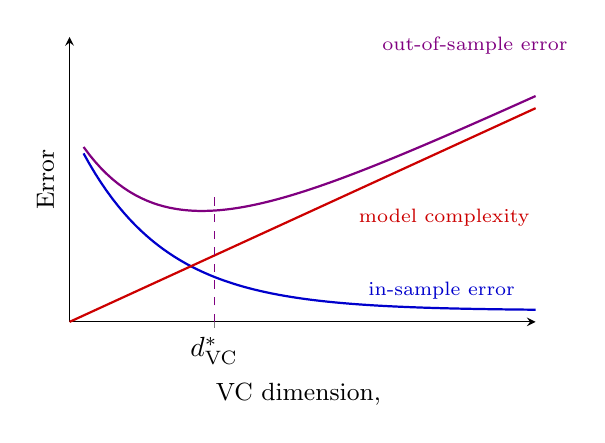
\begin{tikzpicture}
        \begin{axis}[
            width=7.5cm, height=5.2cm,
            xmin=0, xmax=10, ymin=0, ymax=10,
            axis lines=left, xtick={3.1}, xticklabels={\(d_{\mathrm{VC}}^*\)},
            ytick=\empty, xlabel={VC dimension, \(\dvc\)},
            ylabel={Error}, label style={font=\small},
            clip=false]
            \addplot[blue!80!black, thick, domain=0.3:10, samples=80]
                {6.5*exp(-0.55*x) + 0.4};
            \addplot[red!80!black, thick, domain=0:10, samples=40]
                {0.75*x};
            \addplot[Purple, thick, domain=0.3:10, samples=80]
                {6.5*exp(-0.55*x) + 0.4 + 0.75*x};
            \draw[dashed, Purple] (axis cs:3.1,0) -- (axis cs:3.1,4.54);
            \node[font=\scriptsize, text=blue!80!black, anchor=west]
                at (axis cs:6.2,1.1) {in-sample error};
            \node[font=\scriptsize, text=red!80!black, anchor=north west]
                at (axis cs:6.0,4.3) {model complexity};
            \node[font=\scriptsize, text=Purple, anchor=west]
                at (axis cs:6.5,9.7) {out-of-sample error};
        \end{axis}
    \end{tikzpicture}
\end{center}

The picture reads the inequality as a function of \(\dvc\), with the bound
standing in for \(\Eout\):

\begin{itemize}
    \item \(\dvc \uparrow\): \(\Ein \downarrow\) but \(\Omega \uparrow\);
    \item \(\dvc \downarrow\): \(\Omega \downarrow\) but \(\Ein \uparrow\);
    \item best \(d_{\mathrm{VC}}^*\) in the middle.
\end{itemize}

The first bullet is the intuition of \autoref{sec:vc-intuition}: \(\dvc\)
counts the effective binary degrees of freedom, the powerfulness of
\(\mathcal{H}\), and a more powerful \(\mathcal{H}\) can fit the labels
better --- the `Yes!, lots of power' entry of the \(M\)-and-\(\dvc\) table.
But the penalty grows with it, and their sum is smallest somewhere in between.

\begin{remark}
    `More powerful, hence smaller \(\Ein\)' is an intuition, not a fact about
    \(\dvc\) alone. Making it precise takes two assumptions that the picture
    leaves implicit.
    \begin{enumerate}
        \item The hypothesis sets are \emph{nested}: \(\mathcal{H}_1 \subset
            \mathcal{H}_2 \subset \cdots\) with \(\dvc(\mathcal{H}_1) \le
            \dvc(\mathcal{H}_2) \le \cdots\), as when more weights are added to
            a perceptron (setting the new ones to \(0\) recovers the old
            hypotheses).
        \item \(\mathcal{A}\) returns the \(g\) of smallest \(\Ein\) in
            \(\mathcal{H}\).
    \end{enumerate}
    Under these,
    \[
        \min_{h \in \mathcal{H}_2} \Ein(h) \le \min_{h \in \mathcal{H}_1}
        \Ein(h) ,
    \]
    since the best hypothesis of \(\mathcal{H}_1\) is still available in
    \(\mathcal{H}_2\). A larger \(\dvc\) means more dichotomies on the data,
    so a better match to \(y_1, \dots , y_N\) is usually found and the
    inequality is usually strict. Without nesting there is no such guarantee:
    on three collinear inputs labelled \(\times\,\circ\,\times\), positive
    intervals along that line (\(\dvc = 2\)) reach \(\Ein = 0\), while 2D
    perceptrons (\(\dvc = 3\)) cannot.
\end{remark}

\begin{moral}
    Powerful \(\mathcal{H}\) not always good!
\end{moral}

\subsection{VC Bound Rephrase: Sample Complexity}

The same bound can be solved for \(N\) instead. Given specs \(\epsilon = 0.1\),
\(\delta = 0.1\), \(\dvc = 3\), we want
\[
    4 (2N)^{\dvc} \exp \left( -\frac{1}{8} \epsilon^2 N \right) \le \delta .
\]
No closed form, but tabulating the left-hand side is enough:

\begin{center}
    \solidrules
    \begin{tabular}{@{}r|l@{}}
        \toprule
        \(N\) & bound\\
        \midrule
        \(100\) & \(2.82 \times 10^{7}\)\\
        \(1{,}000\) & \(9.17 \times 10^{9}\)\\
        \(10{,}000\) & \(1.19 \times 10^{8}\)\\
        \(100{,}000\) & \textcolor{orange!85!black}{\(1.65 \times 10^{-38}\)}\\
        \(29{,}300\) & \textcolor{orange!85!black}{\(9.99 \times 10^{-2}\)}\\
        \bottomrule
    \end{tabular}
\end{center}

For small \(N\) the polynomial factor wins and the `probability' bound is in
the millions; the exponential only takes over between \(10^4\) and \(10^5\),
and the spec is first met around \(N = 29{,}300\). This gives the
\vocab{sample complexity}: need \(N \approx 10{,}000\, \dvc\) in theory.

\begin{moral}
    Practical rule of thumb: \(N \approx 10\, \dvc\) often enough!
\end{moral}

\subsection{Looseness of VC Bound}

\[
    \mathbb{P}_{\mathcal{D}}\left[ \abs{\Ein(g) - \Eout(g)} > \epsilon \right]
    \le 4 (2N)^{\dvc} \exp \left( -\frac{1}{8} \epsilon^2 N \right)
\]
Theory: \(N \approx 10{,}000\, \dvc\); practice: \(N \approx 10\, \dvc\).

\begin{question}
    Why is the VC bound so loose?
\end{question}

Every step of the derivation paid for generality:

\begin{center}
    \solidrules
    \begin{tabular}{@{}l|l@{}}
        \toprule
        step & it must hold for\\
        \midrule
        Hoeffding for unknown \(\Eout\) & any distribution, any target\\
        \(m_{\mathcal{H}}(N)\) instead of \(\abs{\mathcal{H}(\bm{x}_1, \dots ,
        \bm{x}_N)}\) & `any' data\\
        \(N^{\dvc}\) instead of \(m_{\mathcal{H}}(N)\) & `any' \(\mathcal{H}\) of
        same \(\dvc\)\\
        union bound on worst cases & any choice made by \(\mathcal{A}\)\\
        \bottomrule
    \end{tabular}
\end{center}

--- but hardly better, and `similarly loose for all models'. Tightening one
step usually means assuming something about \(P\), \(f\), the data or
\(\mathcal{A}\), which gives up the very generality that made the bound useful.
And because the looseness is roughly the same for every model, the bound still
ranks models correctly even when its numbers are useless.

\begin{moral}
    Philosophical message of VC bound: important for improving ML.
\end{moral}

\begin{exercise}[Fun Time]
    Consider the VC bound below. How can we decrease the probability of getting
    BAD data?
    \[
        \mathbb{P}_{\mathcal{D}}\left[ \abs{\Ein(g) - \Eout(g)} > \epsilon
        \right]
        \le 4 (2N)^{\dvc} \exp \left( -\frac{1}{8} \epsilon^2 N \right)
    \]
    \begin{enumerate}[(1)]
        \item decrease model complexity \(\dvc\);
        \item increase data size \(N\) a lot;
        \item increase generalization error tolerance \(\epsilon\);
        \item all of the above.
    \end{enumerate}
\end{exercise}

\begin{proof}[Reference Answer]
    (4). Congratulations on being Master of VC bound! :-) Each of (1)--(3)
    shrinks the right-hand side; `a lot' in (2) because the polynomial factor
    grows with \(N\) too, and only wins once \(N\) is large (the table above).
\end{proof}

\hrulebar

\subsection*{Summary}

\begin{description}
    \item[Definition of VC Dimension] maximum non-break point.
    \item[VC Dimension of Perceptrons] \(\dvc(\mathcal{H}) = d + 1\).
    \item[Physical Intuition of VC Dimension] \(\dvc \approx \#\)free
        parameters.
    \item[Interpreting VC Dimension] loosely: model complexity \& sample
        complexity.
\end{description}

Learning happens if \(\dvc\) is finite, \(N\) is large and \(\Ein\) is low. All
of that was derived for the cleanest possible setting: binary classification
with a deterministic target and no noise. Next: more than noiseless binary
classification?
